\chapter[Metodoloxía]{
  \label{chp:metodoloxia}
  Metodoloxía
}
\minitoc
\newpage

Este capítulo pretende explicar as metodoloxías aplicadas durante as diferentes fases do traballo. Nas primeiras etapas seguiuse a metodoloxía TDD (Test Driven Development) e máis adiante optouse por unha metodoloxía XP (Extreme Programming) aínda que, ao ser este un traballo individual, non se aplicaron todas as súas características. Ámbalas dúas poden considerarse metodoloxías áxiles de desenvolvemento iterativo e incremental.

\section{TDD}

Test Driven Development é unha metodoloxía áxil de desenvolvemento que segue a filosofía \say{probar primeiro}. Esta baséase na conversión dos requirimentos en probas antes da propia existencia de código que as avale. Isto obriga ao desenvolvedor a pensar nos requirimentos con detemento, identificar de antemán os posibles fallos e aumentar o alcance da validación de datos. Unha vez o test está definido, pasaremos a implementación da funcionalidade posta a proba. De pasar a proba, repítese co seguinte requirimento. Este ciclo pode verse no esquema da figura \ref{fig:tdd}.

\begin{figure}[h]
	\centering
	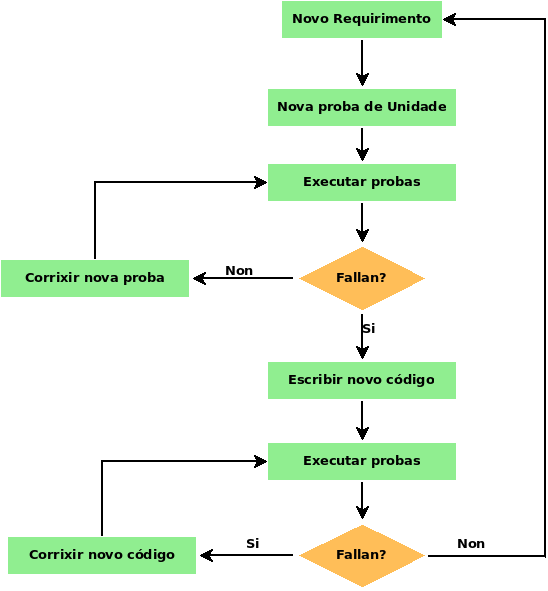
\includegraphics[scale=0.55,keepaspectratio=true]{./images/TDD.png}
	\caption{Diagrama do ciclo de desenvolvemento coa metodoloxía TDD.}
	\label{fig:tdd}
\end{figure}

Existen distintas estratexias á hora de seguir o citado ciclo \cite{tdd} que se poden utilizar en función das características do requirimento:

\begin{itemize}
	\item \textbf{Fake it ('til you make it):} Ou \say{falséao (ata que o fagas)}. Baséase en escribir primeiro un método falso que devolva un valor constante que satisfaga o test. A partir de aí, ilo modificando aos poucos sempre vixiando que o test sexa positivo até que o método estea completo. Esta práctica é moi complexa de utilizar se os métodos son grandes, polo que pode ser unha boa forma de forzar a división, algo desexable para a cualidade do código.
	
	\item \textbf{Triangulación:} Consiste en facer as mesmas comprobación 2 ou máis veces con parámetros distintos dos que esperemos unha saída distinta coa fin de abstraer a función a implementar a raíz dos resultados esperados. Esta implementación é útil para evitar os parámetros superfluos que poidan aparecer nas funcións complexas.
	
	\item \textbf{Implementación Obvia:} Para as funcionalidades sinxelas, non paga a pena utilizar estratexias de abstracción. Podemos simplemente implementar o método e agardar a que o test non falle. Queda a discreción do desenvolvedor definir que funcións son sinxelas e complexas.
	
	\item \textbf{Un a Moitos:} No caso daqueles métodos que actúan sobre unha pluralidade de obxectos, esta estratexia avoga por dividir o requirimento en dous: Habería que validar primeiro o un método que actuaría sobre unicamente un obxecto e, a continuación, validar que se execute sobre dita colección.  

\end{itemize}


Neste proxecto, seguiuse maioritariamente a terceira estratexia da anterior lista por resultar máis intuitiva para o traballo a realizar.

\section{XP}

Extreme Programming, ou Programación Extrema, é un estilo de desenvolvemento de software que promove unha serie de valores de cara ao traballo en equipo e unha serie de técnicas que supoñen unha simplificación e unha alternativa flexible en contraposición a outras metodoloxías máis tradicionais coma, por exemplo, o \say{desenvolvemento en fervenza}.

Eses valores enuméranse coma\cite{xp}: 

\begin{itemize}
	\item \textbf{Comunicación:} Tanto entre programadores coma co cliente.
	\item \textbf{Simplicidade:} Que o código sexa lexible e a documentación concisa.
	\item \textbf{Retroalimentación:} Realizar iteracións curtas para obter opinións rápidas sobre os progresos.
	\item \textbf{Coraxe:} Aceptar que a aparición de novos requirimentos é natural e poden redefinir o deseño.
	\item \textbf{Respecto:} Estrutura horizontal do equipo de desenvolvemento.
\end{itemize}


A posta en práctica dos anteriores valores lévanos a unha metodoloxía de traballo baseada no contacto continuo co cliente para poder obter correccións e ideas novas (retroalimentación). Isto acádase mediante ciclos curtos de desenvolvemento, ao final dos cales volveremos reunirnos co usuario obxectivo e o ciclo volve a comezar. 

Referímonos a estes ciclos coma \say{iteracións}. Poden ser tomadas coma unha planificación do traballo a curto prazo a entender non coma unha improvisación, senón coma unha peza dun plan global suxeito á evolución do proxecto.

Debido á aceptación de que os sucesivos cambios no deseño son inevitables (coraxe) e que a refactorización de código é algo necesario para asegurar a súa cualidade (simplicidade), faise necesaria a automatización de probas e a utilización dun control de versións.

A metodoloxía XP ten unha serie de características aplicables ao traballo en equipo que non se levaron a cabo neste proxecto: A programación por parellas, a revisión de código entre desenvolvedores ou a división do traballo en función da especialización do persoal (Testers, deseñadores de interacción, directores do proxecto, programadores...)